% Chapter 3

\chapter{Continuous Integration and Continuous Delivery} % Main chapter title

\label{Chapter3} % For referencing the chapter elsewhere, use \ref{Chapter1} 

The preparatory work is introduced in this chapter which showcases the process of CI and CD. The chapter commences with a brief introduction about a portfolio of DevOps tools, in use within the department and highlights their importance in development and operation in the Information Technology (IT) industry (see Section~\ref{section:Integrationtools}). Subsequently, an important part of the development process or the background of the Pipeline methodology is explained in Section~\ref{section:CICDpipeline}. Section~\ref{section:ImplementationOutline} presents a detailed implementation outline of the preliminary work done in this research. It is worth noting that all the tools mentioned in this chapter and the paper, in general, are either open-sourced or licensed under the Bosch group. With this chapter, an answer to the following question is presented.

\vspace{0.2cm}
\noindent Question 1: How to automate the process of software integration and delivery ?

%----------------------------------------------------------------------------------------

\section{Portfolio Tools} \label{section:Integrationtools}

\subsection{Version Control} \label{section:versioncontrol}

A tool that manages and tracks different versions of a software or other content is generically referred to as a \ac{VCS}, a Source Code Manager (SCM), a \ac{RCS}, and several other permutations of the word "revision", "version", "code", "content", "control", "management", and "system"~\parencite{loeliger2012version}. A version control is the most effective way of tracking projects which include several developers, performing multiple revisions with collaborative development every day. 

It improves code reproducibility by maintaining versions and revisions of the same software package. There are bunch of hosted version control system platforms like GitHub, GNU Bazaar, Mercurial, SVN which are used in the industry. Among these, GitHub platform is particularly the most popular open source version control system which works perfectly with the illustration of the \ac{CI} \ac{CD} Pipeline concept presented at a later stage in this chapter.

%----------------------------------------------------------------------------------------

\subsection{Jenkins} \label{section:Jenkins}
 
In the context to DevOps, Jenkins, a popular open-source automation server that orchestrates the entire process of software integration and delivery. With numerous plugins available in its marketplace, it becomes highly extensible. Jenkins has a concept of Pipeline to define the stages of execution. A \emph{Jenkins Pipeline} is simply a set of sequential or parallel jobs or both. These jobs can be configured via the GUI, and are defined to perform a set of task. 

Developers can also define the Pipeline as code and save it in a special file (known as Jenkinsfile) in the codebase of the source control repository along with the source code. The practice of defining the Pipeline job as code is known as \emph{Pipeline-as-Code}~\parencite{pathania2017pro}. A \emph{Jenkinsfile} specifies the Pipeline definition and the execution stages. It can be either written in \emph{Groovy} script (Groovy \ac{DSL}) or as a \emph{Declarative Pipeline Syntax}. The syntax which uses the Groovy code is referred as the \emph{Scripted Pipeline Syntax}. A Declarative Pipeline syntax is newly introduced and it is comparatively modern with added flexibility for conditional usage and environment variables. The syntax for both the script only differs a little.
To achieve the goal of the thesis, the in-focus application is also integrated using the Pipeline methodology provided by Jenkins.

%----------------------------------------------------------------------------------------
\subsection{Docker ecosystem}

The concept of \emph{Containerization} is introduced in the industry for its effectiveness to create and deploy application fast. It uses software containers to achieve complete isolation of applications and run different applications within a single host \ac{OS}. Without containerization, isolation of application can be achieved with the help of \emph{Virtualization} or virtual machines~\parencite{leszko2017continuous}. But a virtual machine requires lot of resources and the desktop performance becomes significantly low. The biggest advantage of containerization is the deployment of application using containers and there is no need for a virtual machine. Containers are like a lightweight virtual machine that sets up a computational environment, including all necessary tools, configurations and code within a single unit called image~\parencite{cito2016using}. 

\emph{Docker} is an open-source platform that uses containerization techniques. It is designed for packaging and deploying applications anywhere. A Docker image holds the application with all the dependencies, binaries, and other configurations needed to run it and a Docker container is just a running instance of the image. The size of a Docker image is comparatively much smaller than a virtual machine image.  In today’s software development, containers improve the productivity by packaging applications into portable deployable units~\parencite{benedicic2019sarus}. This ultimately fastens the development and the deployment process of a certain application.

%----------------------------------------------------------------------------------------
\section{Groundwork Preparation for Software Test Suites}

Software testing is a broad spectrum area and inevitable for most companies to validate feature implementations or new enhancements before a software release. In \ac{SDLC}, the \ac{QA} phase plays a major role~\parencite{nidhra2012black}. Indeed, it is a term used in the industry, which includes lot of different approaches. In a general study by Beizer in his book~\parencite{beizer2003software}, he mentions that testing adds up to approx fifty percent of the development cost. This gives an idea about the necessity of testing applications. For instance, there has been an increase amount of interest on "Test and Analysis" topic in recent software conference sessions~\parencite{4221614}.

Likewise, the software components implemented within Bosch also goes through quality checks, passing all the test or validation suites intended for a particular software. Since, all the client based projects are ideally time bounded, a manual test of each components would not be a great solution to validate its effectiveness and henceforth the introduction to automated testing. The main goal of test automation is to minimize the manual efforts as much as possible but simultaneously verify the quality of a particular software or application to detect potential errors. Before the development phase of the \ac{CI} \ac{CD} implementation, a preparatory work was carried away to define all the test cases to validate an in-focus software component (the \ac{REST} \ac{API} application) with Robot test automation framework. The \ac{REST} \ac{API} application has been implemented for the target hardware and helps interact with the backend device through interface. It uses the normal HTTP methods like GET, PUT, POST, DELETE for resources and the message payload is send or received in the form of a \ac{JSON} format. So, in order to validate the payload, status code, and other functionalities, the need for test strategy is prominent. The test suite is defined to perform bulk testing of the \ac{API}'s to detect any potential error and rectify accordingly. Detection at an early stage reduces the rate of software defects at multiple stages of development ~\parencite{asha2015api}.

%----------------------------------------------------------------------------------------
\section{Background}\label{section:CICDpipeline}

The iterative process of software integration have been further accelerated with the introduction of an automated build Pipeline. With the help of an automated Pipeline, the source code is compiled and transformed into binaries and installers. A series of tests runs on the resulting binaries to determine whether a particular release candidate is fit for production release. Traditionally, the point of software release was dealt with stress. But, by adopting the techniques of automated build, test and deployment, developers have the ability to verify changes across a range of environments, and eliminate even a slightest chance of production errors~\parencite{humble2010continuous}.


The implementation background presented in this section utilizes all the functionalities of Jenkins (see Section~\ref{section:Jenkins}), which is best suited among other CI servers. The main purpose behind configuring a Pipeline is to orchestrate the process of software build with quality checks. As presented in the listing \ref{lst:listing-Jenkinsfile}, an example Jenkinsfile is shown which define the Pipeline structure. The Pipeline script consists of multiple code blocks to describe specific jobs. It uses the \texttt{pipeline} directive to include the stages of execution. With the \texttt{stages} directive, the sequential stages are defined. For example, as shown in the listing, the \texttt{Application Build}, \texttt{Test} and \texttt{Deploy to artifactory} are meant to define various phases of execution. The stages uses the \texttt{steps} directive to execute shell tasks. With individual task defined with shell scripts for each stages, the content of Jenkinsfile is kept minimal. Detection of a single failure in either step would cause the entire Pipeline to fail~\parencite{soni2015end}. To configure the build Pipeline in the project, the Jenkinsfile is committed to the root of the source control repository.

\vspace{0.5cm}
\lstset{style=mystyle}
\lstinputlisting[caption= An example Jenkinsfile structure that serves the basic function of defining the execution stages of a Pipeline, captionpos=b,   basicstyle=\footnotesize, stepnumber=1, frame=lines, numbers=left, label={lst:listing-Jenkinsfile}, language=python]{code/Jenkinsfile}
\vspace{0.5cm}

The source code runs through each stages of the Pipeline, resulting in failure if there is any potential error detected in any step. With a success, an output in the form of a deployment artifact is generated as the result of the build process. A \emph{deployment artifact} in \ac{CI} \ac{CD} systems represents a packaged application or module that is ready to be deployed~\parencite{railic2021architecting}. To get a clear overview of the implemented scripts defined in each stages of the Pipeline, an example is shown in listing \ref{lst:listing-DeploymentScript} where it outlines the sample deploy script written in shell command language to define the final deployment stage of software package test reports. Here, the target artifactory address and the authenticated user credentials are defined with respective variables(line 10 to 13), needed by the \texttt{curl} method for the file transfer. The execution body contains several validation checks (line 16 to 23) to determine a correct target location and the transfer status.



\vspace{0.5cm}
\lstset{style=mystyle}
\lstinputlisting[caption= The A sample bash script to define the deployment of test reports, captionpos=b,   basicstyle=\footnotesize, stepnumber=1, frame=lines, numbers=left, label={lst:listing-DeploymentScript}, language=bash]{code/deploymenttestreports.sh}
\vspace{0.5cm}



To reach the goal of this thesis, the actual work focuses on the test report deployment artifact of the in-focus software application packaged to a \texttt{".rar"} file. It gets deployed into the JFrog artifact repository. The deployed artifact should indicate the release version to identify which version of the software component is tested against.


\section{Implementation Outline}\label{section:ImplementationOutline}

Based on the portfolio of tools presented in Section~\ref{section:Integrationtools}, and the implementation background outlined in Section~\ref{section:CICDpipeline}, the solution space for the Jenkins Pipeline implementation is explored. The described tools work as a combined unit in Pipeline job. The Pipeline covers the collective stages of \ac{CI} \ac{CD} implementation and can be configured in various ways.


At the initial phase, the project repository hosted via the GitHub platform is configured with the source code files of the in-focus software package, the automated test suites, Jenkinsfile, and other essential scripts, needed to define the different stages of the Pipeline. Besides, the version control repository keeps track of every initial development versions with the help of software version numbers, configured with git tags. This aid to better tracking of every changes committed to the project codebase. For a better understanding of the concept of software release and its benefits, this thesis also presents a seamless way to handle software version (See Chapter \ref{Chapter 4}). The configured Jenkinsfile is written using the Declarative Pipeline syntax and covers all the sequential stages of build, test and deployment. Additionally, the Jenkins server, used for other software development projects within the Bosch, is configured with a new \emph{Multibranch Pipeline} item which sets the required Pipeline job. With an execution of the build, the project repository is checked out. The following process flow diagrams illustrates a detailed outline of the individual build stages, configured to achieve the preparatory work of software build, running the test suites and deploying the test reports. Due to the sequential arrangement of multiple stages and better understandability, the control flow is seems split-up but it is continuous across different stages (see arrows).


%----------------------------------------------------------------------------------------
\vspace{0.5cm}
\begin{figure}[H]
\begin{tikzpicture}[node distance=1.5cm,
    every node/.style={fill=white, font=\sffamily}, align=center]
  % Specification of nodes (position, etc.)
  \node (start)             [activityStarts, drop shadow] {Source control repository (Jenkinsfile, Source Code, Test Suites)};
    \node (onCreateBlock)     [process, drop shadow, below of=start]          {\ac{CI} Pipeline};
        \node (onCheckoutBlock)     [process, drop shadow, below of=onCreateBlock]          {SCM (Source Code Management) checkout};
        \node (beg)      [below of=onCheckoutBlock]   {};
  \draw[->]             (start) -- (onCreateBlock);
  \draw[->]             (onCreateBlock) -- (onCheckoutBlock);
  \draw[->]     (onCheckoutBlock) -- (beg);
  
\end{tikzpicture}
\caption [Configuration of the project’s source control repository]{The source control repository is configured with a Jenkinsfile to define the entire build process}
\end{figure}
%----------------------------------------------------------------------------------------

%covers how Jenkins can invoke Docker containers on agents/nodes (from a Jenkinsfile) to build your Pipeline projects,
At the build stage, multiple container applications are invoked with the \emph{Docker Compose} tool. A docker container runs an instance of a docker image either taken directly from docker hub, or configuring a custom docker image with all the system and application requirements. If there is a need to set a custom image, it can handled by defining all the specifications with the help of a \emph{Dockerfile} and building a docker image from it. 

\vspace{0.5cm}
\begin{figure}[H]
\begin{tikzpicture}[node distance=1.5cm, every node/.style={fill=white, font=\sffamily}, align=center]
  \node (onCrBlock)      [above of=onStartBlock]   {};
  \node (onStartBlock)      [process, below of=onCrBlock, drop shadow, yshift=-1cm]   {Docker Compose};
  \node (onResumeBlock)     [process, below of=onStartBlock, drop shadow, yshift=-0.5cm]   {Run the Docker container};
    \node (onRestartBlock)    [process, drop shadow, right of=onStartBlock, xshift=4cm]
                                                              {Multi-Container\\ Applications};
  \node (ActivityEnds)      [startstop, drop shadow, left of=onStartBlock, xshift=-4cm]
                                                        {Dockerfile};
                                                    
    \node (ActivityStr)      [startstop, drop shadow, left of=onResumeBlock, xshift=-4cm]
                                                        {Build Docker image};
    \node (an)      [below of=onResumeBlock, yshift=-0.3cm]   {};
       \draw[->]     (onCrBlock) -- node[text width=4cm]
                                   {Stage: Build}(onStartBlock);
        \draw[->]      (onStartBlock) --  (onResumeBlock);
      \draw[->]    (onRestartBlock) -- (onStartBlock);
     \draw[->]    (ActivityEnds) -- (ActivityStr);
    \draw[->]      (ActivityStr) -- (onResumeBlock);
      \draw[->]     (onResumeBlock) --  (an);
\end{tikzpicture}
\caption [Running the multi-container docker applications]{At the Build stage, the multi-container docker applications are invoked to run on Jenkins agent or machine}
\end{figure}

%----------------------------------------------------------------------------------------

The next stage constitute executing the predefined automated test suites (prepared at the groundwork phase), to validate the intended in-focus application. 

\vspace{0.5cm}
\begin{figure}[H]
\begin{tikzpicture}[node distance=1.5cm,
    every node/.style={fill=white, font=\sffamily}, align=center]
  % Specification of nodes (position, etc.)
\node (onTeBlock) {};
\node (activityRuns)      [process, below of=onTeBlock, drop shadow, yshift=-1cm] {Run Automated Test};
    \node (testFinish)      [below of=activityRuns]   {};
\draw[->]     (onTeBlock) -- node[text width=4cm]
                                   {Stage: Test} (activityRuns);
\draw[->]     (activityRuns) --  (testFinish);
\end{tikzpicture}
\textbf{\caption [Executing automated test suites at the Test stage]{The automated test suites are executed to validate the intended application at the Test stage}}
\end{figure}
%----------------------------------------------------------------------------------------

Following the completion of the Test stage, the final phase of \ac{CD} covers the publish and deployment of test reports into a specific delivery location. Jenkins offers several plugins in its marketplace which helps to publish the test results in the dashboard of a particular Pipeline build job. This thesis utilize the \emph{Robot Framework Jenkins Plugin} to publish the test results in Jenkins, written using Robot Framework. The test results are displayed with the help of a trend graph on a dashboard (see Figure \ref{fig:SampleTrendGraph}). The results dashboard brings better visibility of the software quality with each build.

\vspace{0.5cm}
\begin{figure}[H]
\centering{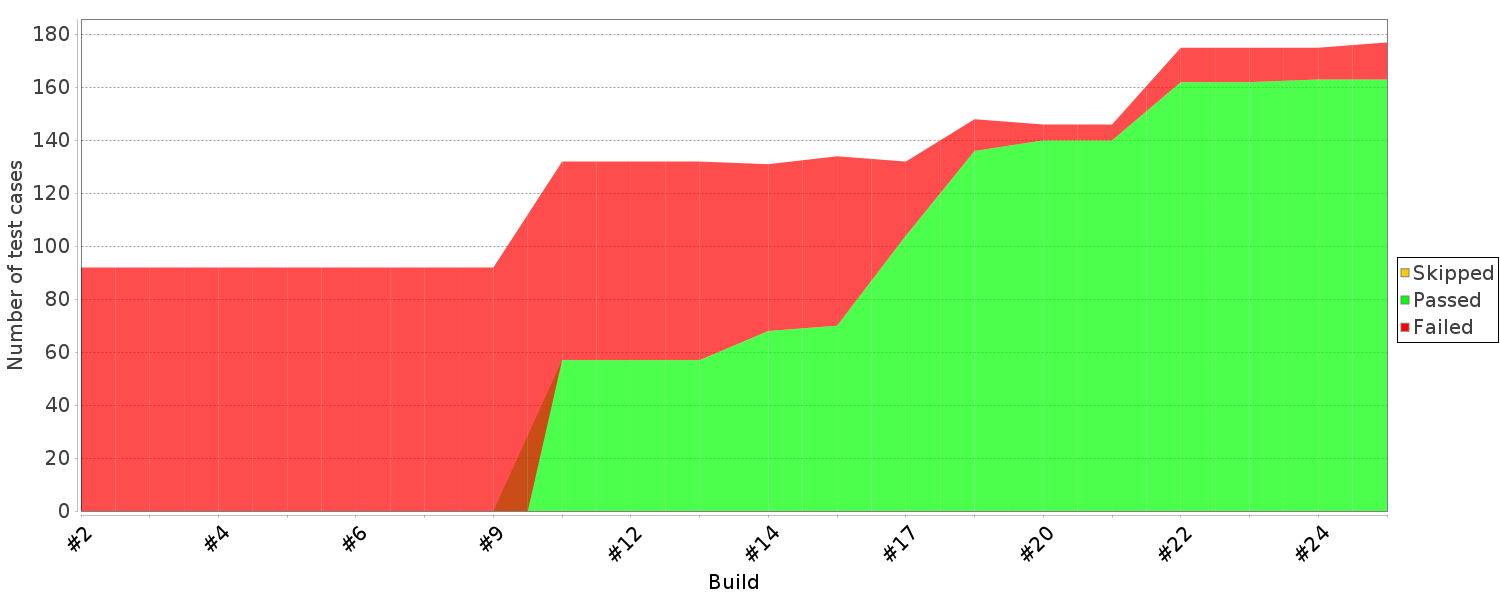
\includegraphics[width=1\textwidth]{figures/trendgraph.png} }%
\caption[An example of the trend graph]{An example trend graph of the test results, published in Jenkins}
\label{fig:SampleTrendGraph}
\end{figure}
\vspace{0.5cm}




At the Deployment stage, the resultant report files are deployed to the \ac{BDC} based JFrog artifact repository. The deployed test reports indicate a proper software release version. Success in the individual stages will lead to the entire Pipeline build process being successful.
%----------------------------------------------------------------------------------------
\vspace{0.5cm}
\begin{figure}[H]
\begin{tikzpicture}[node distance=1.2cm,
    every node/.style={fill=white, font=\sffamily}, align=center]
  % Specification of nodes (position, etc.)
\node (final) {};
  \node (onPauseBlock)      [process, below of=final, drop shadow, yshift=-0.6cm]
                                                                {Publish Test Results};
  \node (onDestroyBlock)    [process, drop shadow, below of=onPauseBlock, yshift=-1.0cm] 
                                                              {JFrog Artifact Repository};
  \node (ActivityDestroyed) [activityRuns, drop shadow, below of=onDestroyBlock, yshift=-0.4cm]
                                                    {Successful Pipeline Build};     
  % Specification of lines between nodes specified above
  % with aditional nodes for description 
  \draw[->]      (final) -- node[text width=4cm]
                                   {Stage: Publish}  (onPauseBlock);
  \draw[->]      (onPauseBlock) -- node[text width=4cm]
                                   {Stage: Deployment} (onDestroyBlock);

  \draw[-]    (onDestroyBlock) -- (ActivityDestroyed);

                                   
\end{tikzpicture}
\caption [The final \ac{CD} stage]{The \ac{CD} stage covers the publish and deployment of test results}
\end{figure}

















\clearpage\null\thispagestyle{empty}